%# -*- coding: utf-8-unix -*-
%%==================================================
%% chapter_2.tex for SJTU Master Thesis
%%==================================================

\chapter{时间序列样本统计方法}
\label{chap:1588_theory}
在本章中,将依据对IEEE1588时钟同步原理及协议中可能存在的一些应用问题进行分析,并梳理关于这些问题的当今研究理论成果来作一个全面的分析。

\section{IEEE1588时钟同步原理}
% IEEE1588协议内部集成了多项分布式技术,如网络通信、局部计算和分布式对象等,对于所有支持多播局域网通信的分布式系统,尤其是以太网,都可以应用PTP协议来进行时钟同步。这可以在占用极少网络和本地计算资源的前提下,使得各类具有不同精确度、分辨率和稳定性的时钟同步且达到亚微秒级别的同步精度。由于当今测控系统中越来越多的依赖分布式系统技术,而分布式系统的性能又极其依靠所有分布式节点之间的时钟同步精度。所以,一套优秀且能达到微秒甚至亚微秒级别的时钟同步协议显得尤为迫切,而IEEE1588协议的出现给这种需求带来了重要的影响,在相关领域也得到了非常快速的发展。

% 下面,详细介绍主从建立过程中及时钟同步过程中所应用到的算法,并对算法进行分析。

% 由于ptp协议的核心是从时钟向主时钟同步从而最终实现整个系统时钟同步。所以,在真正的时钟同步之前,至关重要的一步便是建立全系统主从秩序,在该建立过程中,所有网络节点会通过“最佳主时钟算法(Best Master Clock Algorithm, BMC)”,选举出Grand Master Clock、主时钟、从时钟。其中,Grand Master Clock的精度最高,主时钟其次,从时钟最低。

% 下面进行简明扼要的最佳主时钟算法介绍。

% 当系统在启动之初,所有系统内部的时钟会对外发布Announce报文,该报文会包含自身时钟的与精度相关的特性。与此同时,所有时钟也会接受其他时钟发送过来的Announce报文,即接收到其他报文传递来的精度信息。

% 然后,每个端口内部会依据这些精度相关的数据集,在本地首先通过数据集比较算法,从而比较出两组数据的优劣,其中一组是时钟自身的缺省特性,另一组是来自外界其他时钟传递过来的数据。完成了数据集比较之后,会依靠比较结果继续执行状态决定算法。该算法会结合端口状态机规则及数据集比较结果来设置自身端口的主从状态。至此,每个时钟便已设置好了自身的主从状态,这其中最高级的主时钟便自动成为了Grand Master Clock。

% 具体拓扑结构可以参考下图:
% \\
% \\
% \begin{figure}[htbp]
%   \centering
%   \begin{minipage}[b]{0.6\textwidth}
%     \captionstyle{\centering}
%     \centering
%     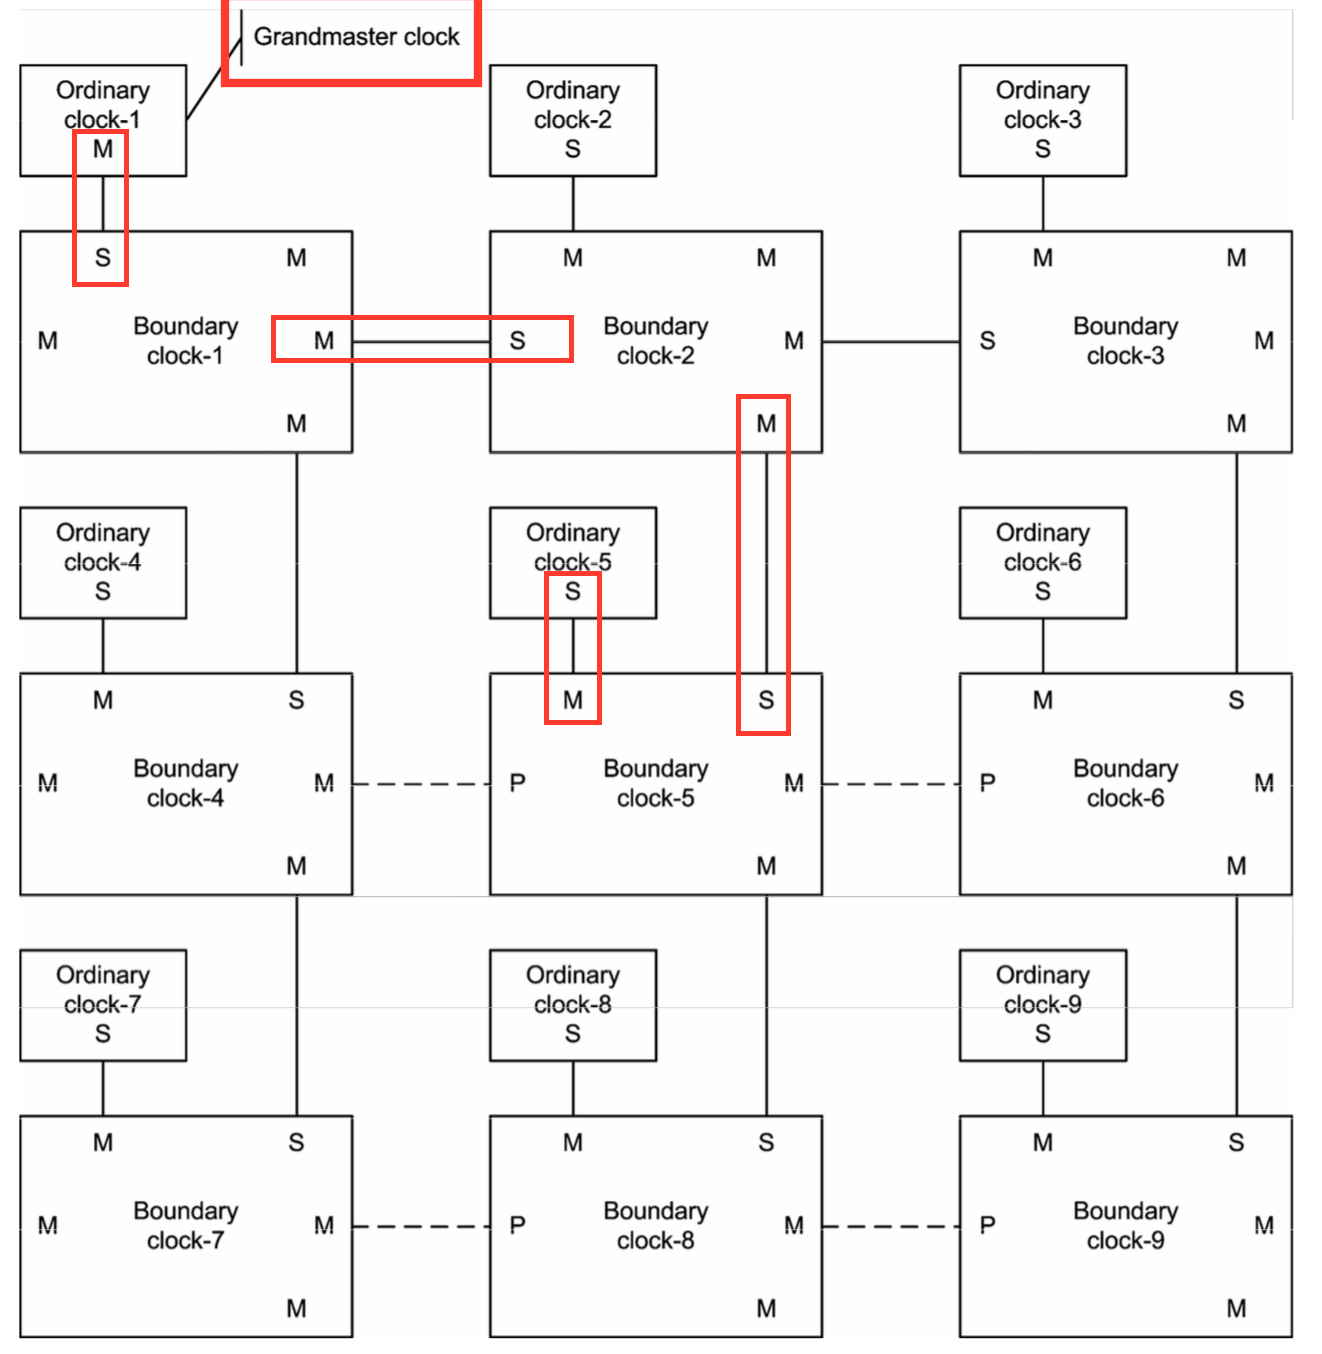
\includegraphics[width=10cm]{ptp_topo}
%     \bicaption[fig:longcaptiongood]{PTP时钟同步拓扑结构}{PTP时钟同步拓扑结构}{Fig}{The topology of PTP Time-Sync System}
%   \end{minipage}     
% \end{figure}

% \subsection{时钟同步算法}
IEEE1588系统是由PTP设备和非PTP设备结合而成的分布式网络化系统。IEEE1588协议主要介绍的是系统中的实时PTP设备之间的相互同步方案,使得所有的从时钟能够与自己的主时钟同步,而所有主时钟又能够和同一个Grand Master时钟同步,最终达到整个系统中所有时钟保持同步。

首先,每个PTP时钟会有多个端口,当系统启动时,会立即开始PTP网络建立过程。该过程中,每个端口会对外发送Announce报文,同时通过检查所收到的Announce报文中的相关信息来判定哪个端口适合成为主时钟,被判定为主时钟的端口则会定期对外发送Sync报文。如果,一个判定为主时钟的端口收到了一个来自于更好的主时钟的Sync报文,那么该主时钟则会立即将自身的主时钟状态切换为从时钟状态。当然,如果一个处于从时钟状态的端口认为自己比当前主时钟更加好,那么它可以将自己设置为主时钟状态,并对外发送Sync报文。当所有端口通过互相比较时钟特性并建立了各自的主从状态后,则意味着主从秩序完成建立。如果此时新加入了一个时钟,那么该时钟首先会等待来自某一主时钟的Sync报文,若在规定的时间内没有收到任何主时钟的Sync报文,那么该时钟则将自身设置为主时钟,直到发现一个更好的主时钟。

随后,则会进行时钟同步过程。该过程主要是主从时钟之间发送报文,使得每个从时钟计算出自身与主时钟之间的时钟偏差,并且对自身进行校正从而实现同步。首先主时钟会对外界进行周期性的Sync报文发送,对于采用硬件时间戳的设备将直接在Sync报文内记录发送时间,否则的话将再发送Follow\_up报文来进行发送。当从时钟收到Sync报文后,则能够接受到发送时间戳并记录当前的接收时间戳。同时,从时钟自身也会周期性向主时钟发送Delay\_Req报文,会通过接受主时钟回传的Delay\_Resp报文来共同计算出链路延时$T_{delay}$和主从偏差$T_{offset}$。最终利用$T_{offset}$对从时钟进行校正而实现同步。
\label{sec:1588_theory_sync}
在图\ref{fig:process_of_time_sync}中,可以看到较为完整的时钟同步过程。下面,对时钟同步过程及相关计算做简明扼要地介绍。

\begin{figure}[htbp]
  \centering
  \begin{minipage}[b]{0.6\textwidth}
    \captionstyle{\centering}
    \centering
    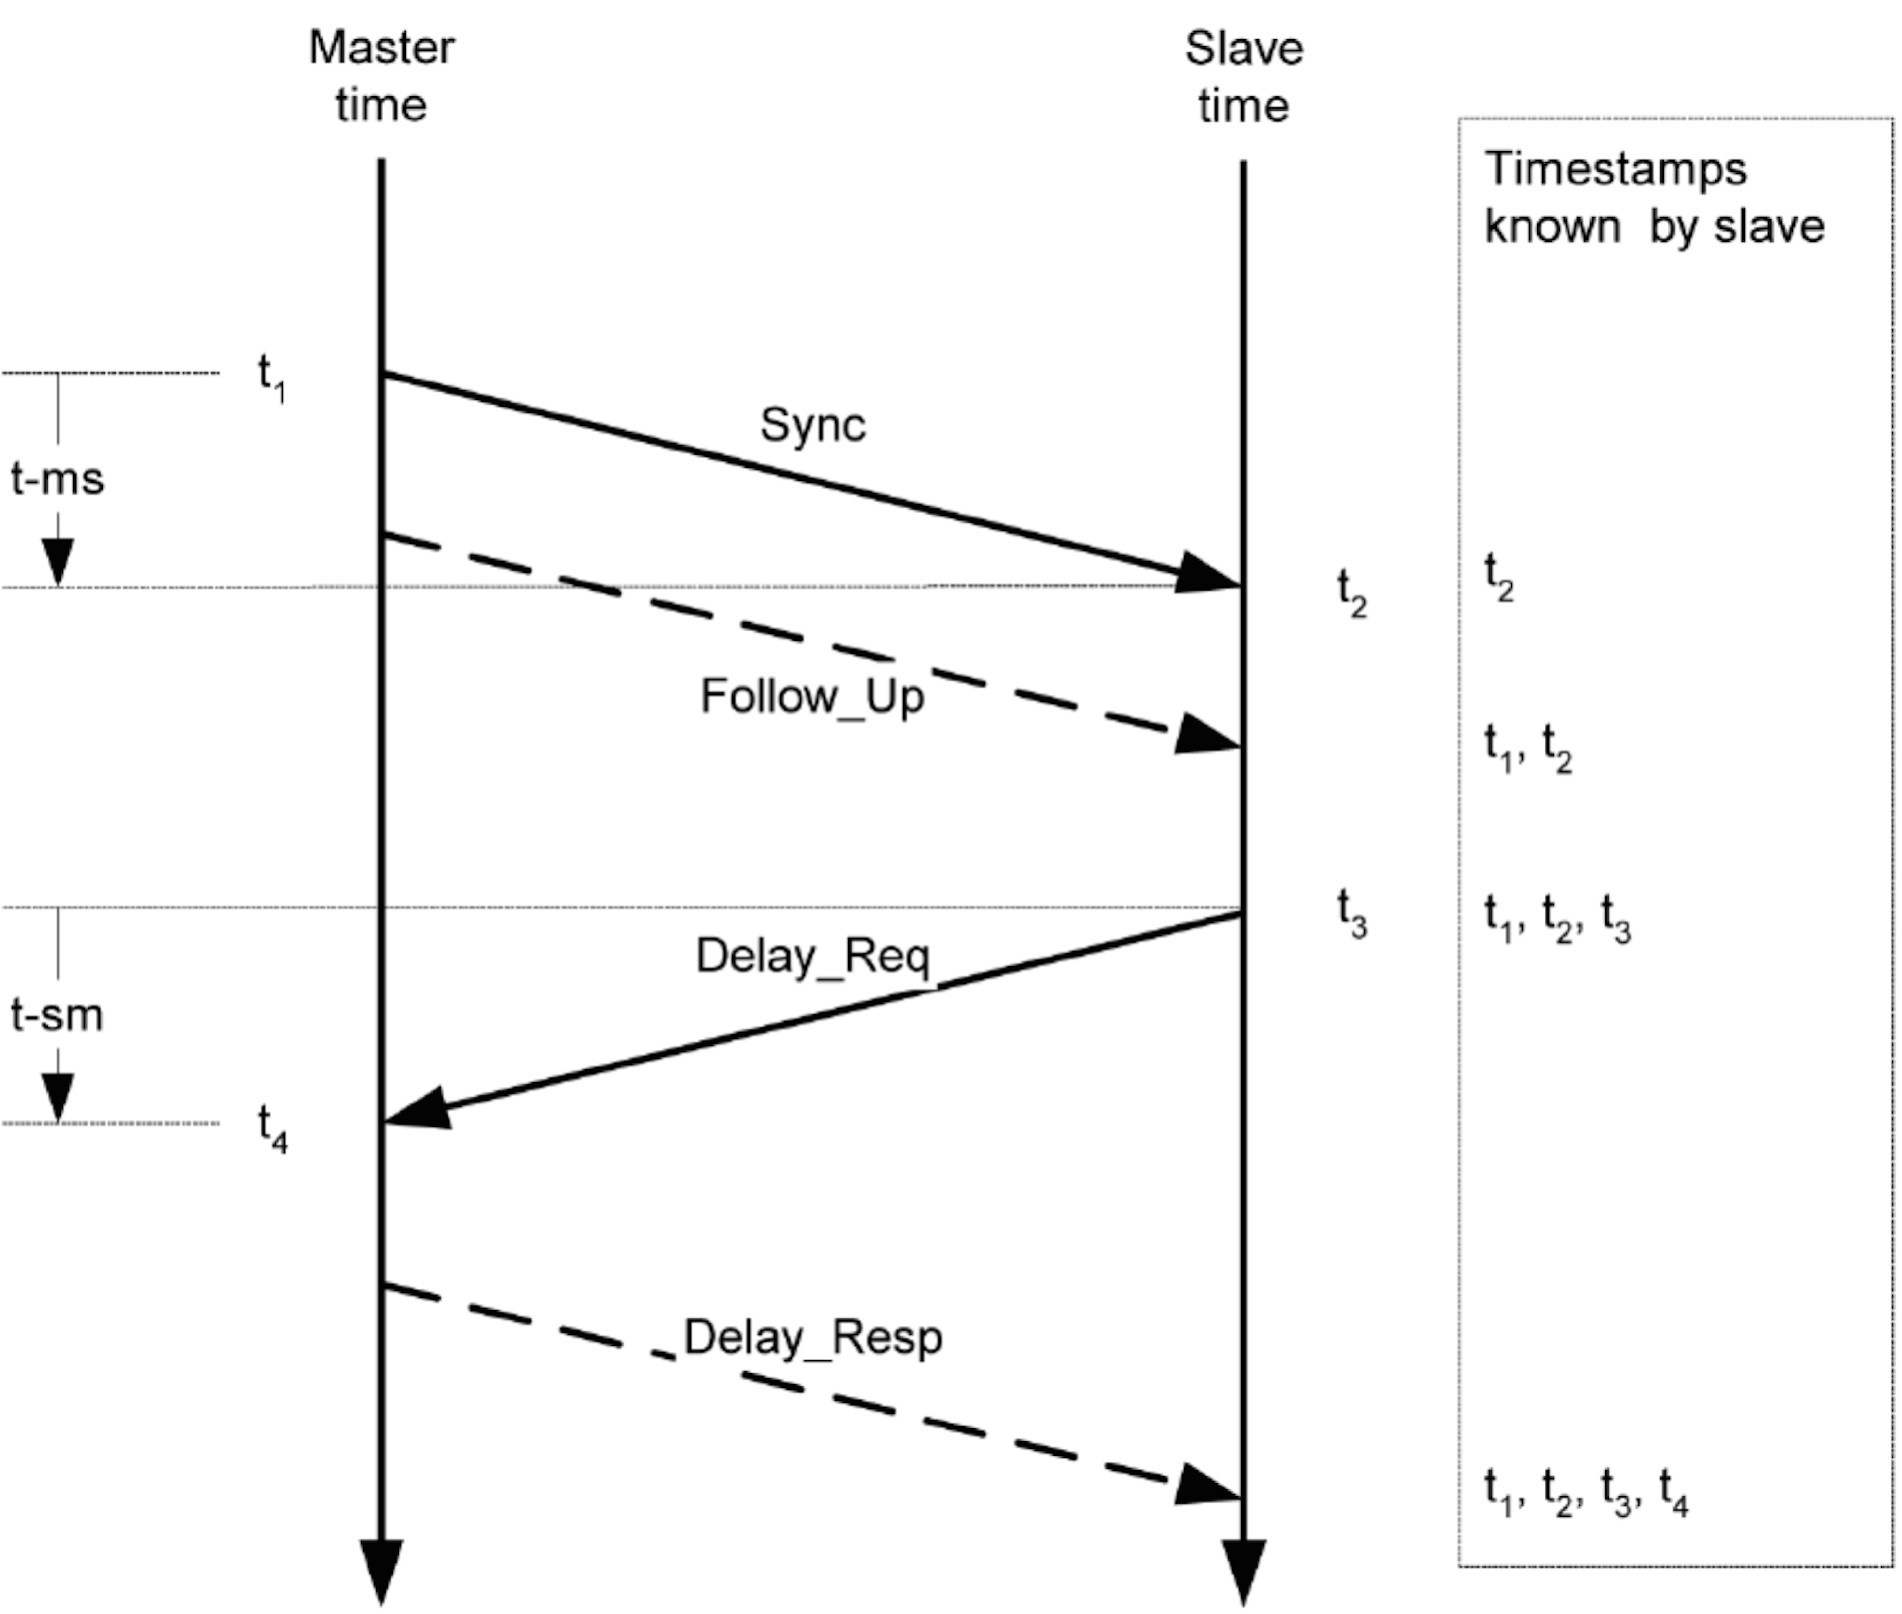
\includegraphics[width=10cm]{process_of_time_sync}
    \bicaption[fig:process_of_time_sync]{时钟同步算法流程图}{时钟同步算法流程图}{Fig}{Method of Time Sync}
  \end{minipage}     
\end{figure}

\subsection{时钟相位调节}
首先,主时钟会周期性对外发送Sync报文,当该报文离开主时钟时会记录时间戳为$t_{1}$。

然后,当从时钟接收到Sync报文时,标记接收时间为$t_{2}$。此时,从时钟即获得了Sync报文的发送与接收时间戳$t_{1}$和$t_{2}$。那么假设主从时间偏差为$T_{offset}$,主从时钟间网络传输时间为$T_{delay}$,则可以得到下面式子:
\begin{align}
	T_{offset} + T_{delay_1} = t_2 - t_1
\end{align}
另外,从时钟周期性向主时钟发送Delay\_Req报文,假设发送时间为$t_{3}$,当主时钟收到该报文时,会立即记录下Delay\_Req报文的接收时间$t_{4}$,并把该接收时间$t_{4}$存入Delay\_Resp报文中传递回该从时钟。那么此时,从时钟会得到$t_{3}$和$t_{4}$两个时间,可得到下面式子:
\begin{align}
	T_{delay_2} - T_{offset} = t_4 - t_3
\end{align}
此时,根据协议标准中,将往返传输延时视为对称,即:
\begin{align}
	T_{delay_1} = T_{delay_2} = T_{delay}
\end{align}
所以,结合上面几个式子可以得到如下结果:
\begin{align}
	T_{delay} = \frac{(t_2 - t_1) + (t_4 - t_3)}{2}
\end{align}
\begin{align}
	T_{offset} = \frac{(t_2 - t_1) - (t_4 - t_3)}{2}
\end{align}

通过上面的计算方法,可以得到主从时钟之间的相位偏差$T_{offset}$。然后,还需要计算主从时钟的时钟频率偏差才能实现完整的时钟同步。

\subsection{时钟频率调节}
在大多数情况下,主时钟设备会采用高稳时钟作为时间源,其频率一般非常稳定。但是,从时钟设备一般只会采用普通晶振源作为时钟源,其物理特性较差,容易受到外界环境和自身寿命等因素导致时钟漂移,这就导致了主从时钟由于频率差异而时时处于变化之中。因此,如果想要实现主从时钟的真正同步,就必须调节从时钟频率以使其保持与主时钟一致,从而缓解同步误差的根本来源。

为了计算时钟频率偏差,假设主时钟是按固定周期向从时钟发送Sync报文,那么,对主时钟而言,第(k-1)个Sync报文和第(k)个Sync报文之间的发送间隔\supercite{6}为:
\begin{align}
	\Delta T_{master} = T_{master(k)} - T_{master(k - 1)}
\end{align}
其中,$T_{master(k)}$表示第k个Sync报文的主时钟发送时间。

对于从时钟而言,两个Sync报文的时间间隔\supercite{6}为:
\begin{align}
	\Delta T_{slave} = T_{slave(k)} - T_{slave(k - 1)}
\end{align}
其中,$T_{slave(k)}$表示第k个Sync报文的在从时钟处的接收时间。由此得到主从时钟的频率偏差。
\begin{align}
	\Delta f = \frac{\Delta T_{master}}{\Delta T_{slave}}
\end{align}
因此,可以对从时钟的晶振设备进行调节,将其本地频率扩大$\Delta f$倍,即可实现主从时钟频率一致。通过不断对从时钟晶振源频率进行调节,可以减小主从时钟的计时速率偏差,从根本上减小了主从时钟偏差的来源。

为了能够采用上述方法来进行频率调节,在实际运行中需要确保主时钟周期性对外发送PTP报文,例如Sync报文,在这样的前提下,从时钟只需要累计一定周期内Sync报文的发送时间和接收时间,利用这些数据可以对主从时钟的频率差进行估计。

% 另外,IEEE1588系统是由PTP设备和非PTP设备结合而成的分布式网络化系统。其中,PTP设备包括普通时钟(Ordinary Clock, OC)、边界时钟(Boundary Clock, BC)、端到端/点到点透明时钟(End-to-End/Peer-to-Peer Transparent Clock, TC)和管理节点。非PTP设备包括普通交换机、路由器及其他底层设备等。

% \begin{itemize}[noitemsep,topsep=0pt,parsep=0pt,partopsep=0pt]
% 	\item 普通时钟(Ordinary Clock, OC):普通时钟只有一个物理PTP端口,内部包含两个逻辑接口:事件接口主要用来收发含有时间戳的事件报文;通用接口主要用来收发不含时间戳的通用报文。普通时钟指网络中的一般节点,比如电信网基站,或者工业中的测量仪器。
% 	\item 边界时钟(Boundary Clock, BC):边界时钟包含一个或多个PTP端口,在物理上将一个同步网络划分为多个子网。其每一个端口相当于一个普通时钟,能够引出一条PTP路径,若该端口连接主时钟,则表现从时钟属性;若连接从时钟,则该端口表现主时钟属性。另外,非PTP报文可以通过它来转发,但PTP报文不可以跨越边界时钟。在实际应用中,边界时钟一般安装在路由器、交换机等具有数据收发功能的网络设备上。
% 	\item 透明时钟(Transparent Clock, TC):透明时钟可以记录报文的进入时间戳和离开时间戳,利用两个时间戳相减得到的相对时间作为驻留时间传递给从时钟,从时钟可以减去该时间从而仿佛报文从未经过该透明时钟,使得波动因素更小。
% 	\item 管理节点(Management Node):管理节点不需要实现时钟同步功能,它只需要能够对时钟同步进行管理。
% \end{itemize}

% PTP协议中的报文分两类,事件(Event)报文和一般(General)报文。下面简单介绍本文使用最多的几种报文。Announce报文主要用于最佳主时钟算法,报文内部包含描述主时钟所需的数据集,当时钟接收到该报文时,即会调用最佳主时钟算法,比较自身与外部时钟的品质,并根据结果来决定端口的主从状态\supercite{52}。然后,主时钟周期性对外发送Sync报文,该报文包含了主时钟发送时的时间戳。当从时钟接收到该报文,就会通过offset计算方法来计算出主从时间偏差,并以此来校正自身从而实现同步\supercite{52}。Delay\_Req和Delay\_Res报文:为了获得主从时钟间的路径传输延时,从时钟会周期性对主时钟发送Delay\_Req报文,当主时钟接收到该报文时,会立即保存接收时间戳,并通过回传Delay\_Res报文把接收时间戳返回给从时钟,用于从时钟的delay值更新\supercite{52}。

% 所有PTP报文头格式一致,各字段含义如下:
% \begin{itemize}[noitemsep,topsep=0pt,parsep=0pt,partopsep=0pt]
% 	\item transportSpecific:标记下一层协议类型,用来区分UDP/IPv6、UDP/IPv4和IEEE802.3;
% 	\item messageType:标记当前PTP报文类型,包括Sync、Delay\_Req、Follow\_Up、Delay\_Req等;
% 	\item versionPTP:标记当前PTP版本;
% 	\item messageLength:标记PTP报文总长度,包含报文头部、报文主体及报文扩展字段;
% 	\item domainNumber:标记PTP发送端口所属域编号;
% 	\item flagField:标记单步或双步模式;
% 	\item correctionField:标记时间修正域,即报文转发时的驻留时间或链路传输延时,该字段为64位有符号整型,意味着它可以使得时间同步精度达到1ns;
% 	\item sourcePortIdentity:标记发送报文的源端口号,由设备ID及端口ID组成。
% \end{itemize}

% Sync和Req\_Delay两种报文主体主要包括了时间戳信息:NanosecondsField和SecondsField,分别表示时间戳的秒部分和纳秒部分。

% \begin{figure}[!hbp]
%   \centering
%   \begin{minipage}[b]{0.6\textwidth}
%     \captionstyle{\centering}
%     \centering
%     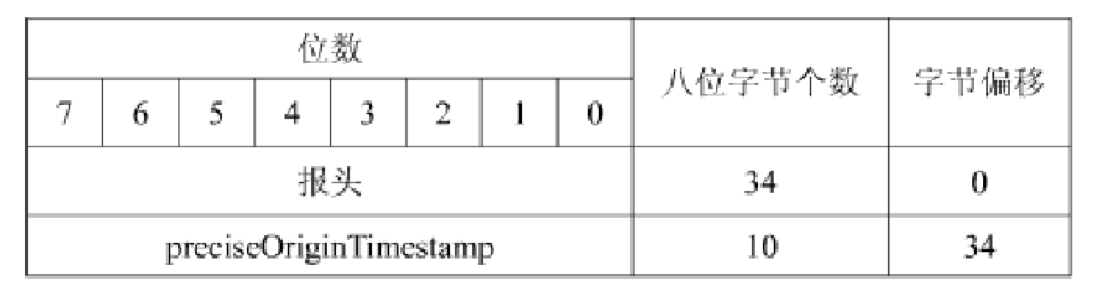
\includegraphics[width=10cm]{ptp_message_content}
%     \bicaption[fig:longcaptiongood]{PTP报文主体格式}{PTP报文主体格式}{Fig}{The Structure of Sync Req\_Delay message content}
%   \end{minipage}     
% \end{figure}

% 另外,对于Announce报文,其主体内容如图\ref{fig:ptp_announce_message_content}所示:

% \begin{figure}[htbp]
%   \centering
%   \begin{minipage}[b]{0.6\textwidth}
%     \captionstyle{\centering}
%     \centering
%     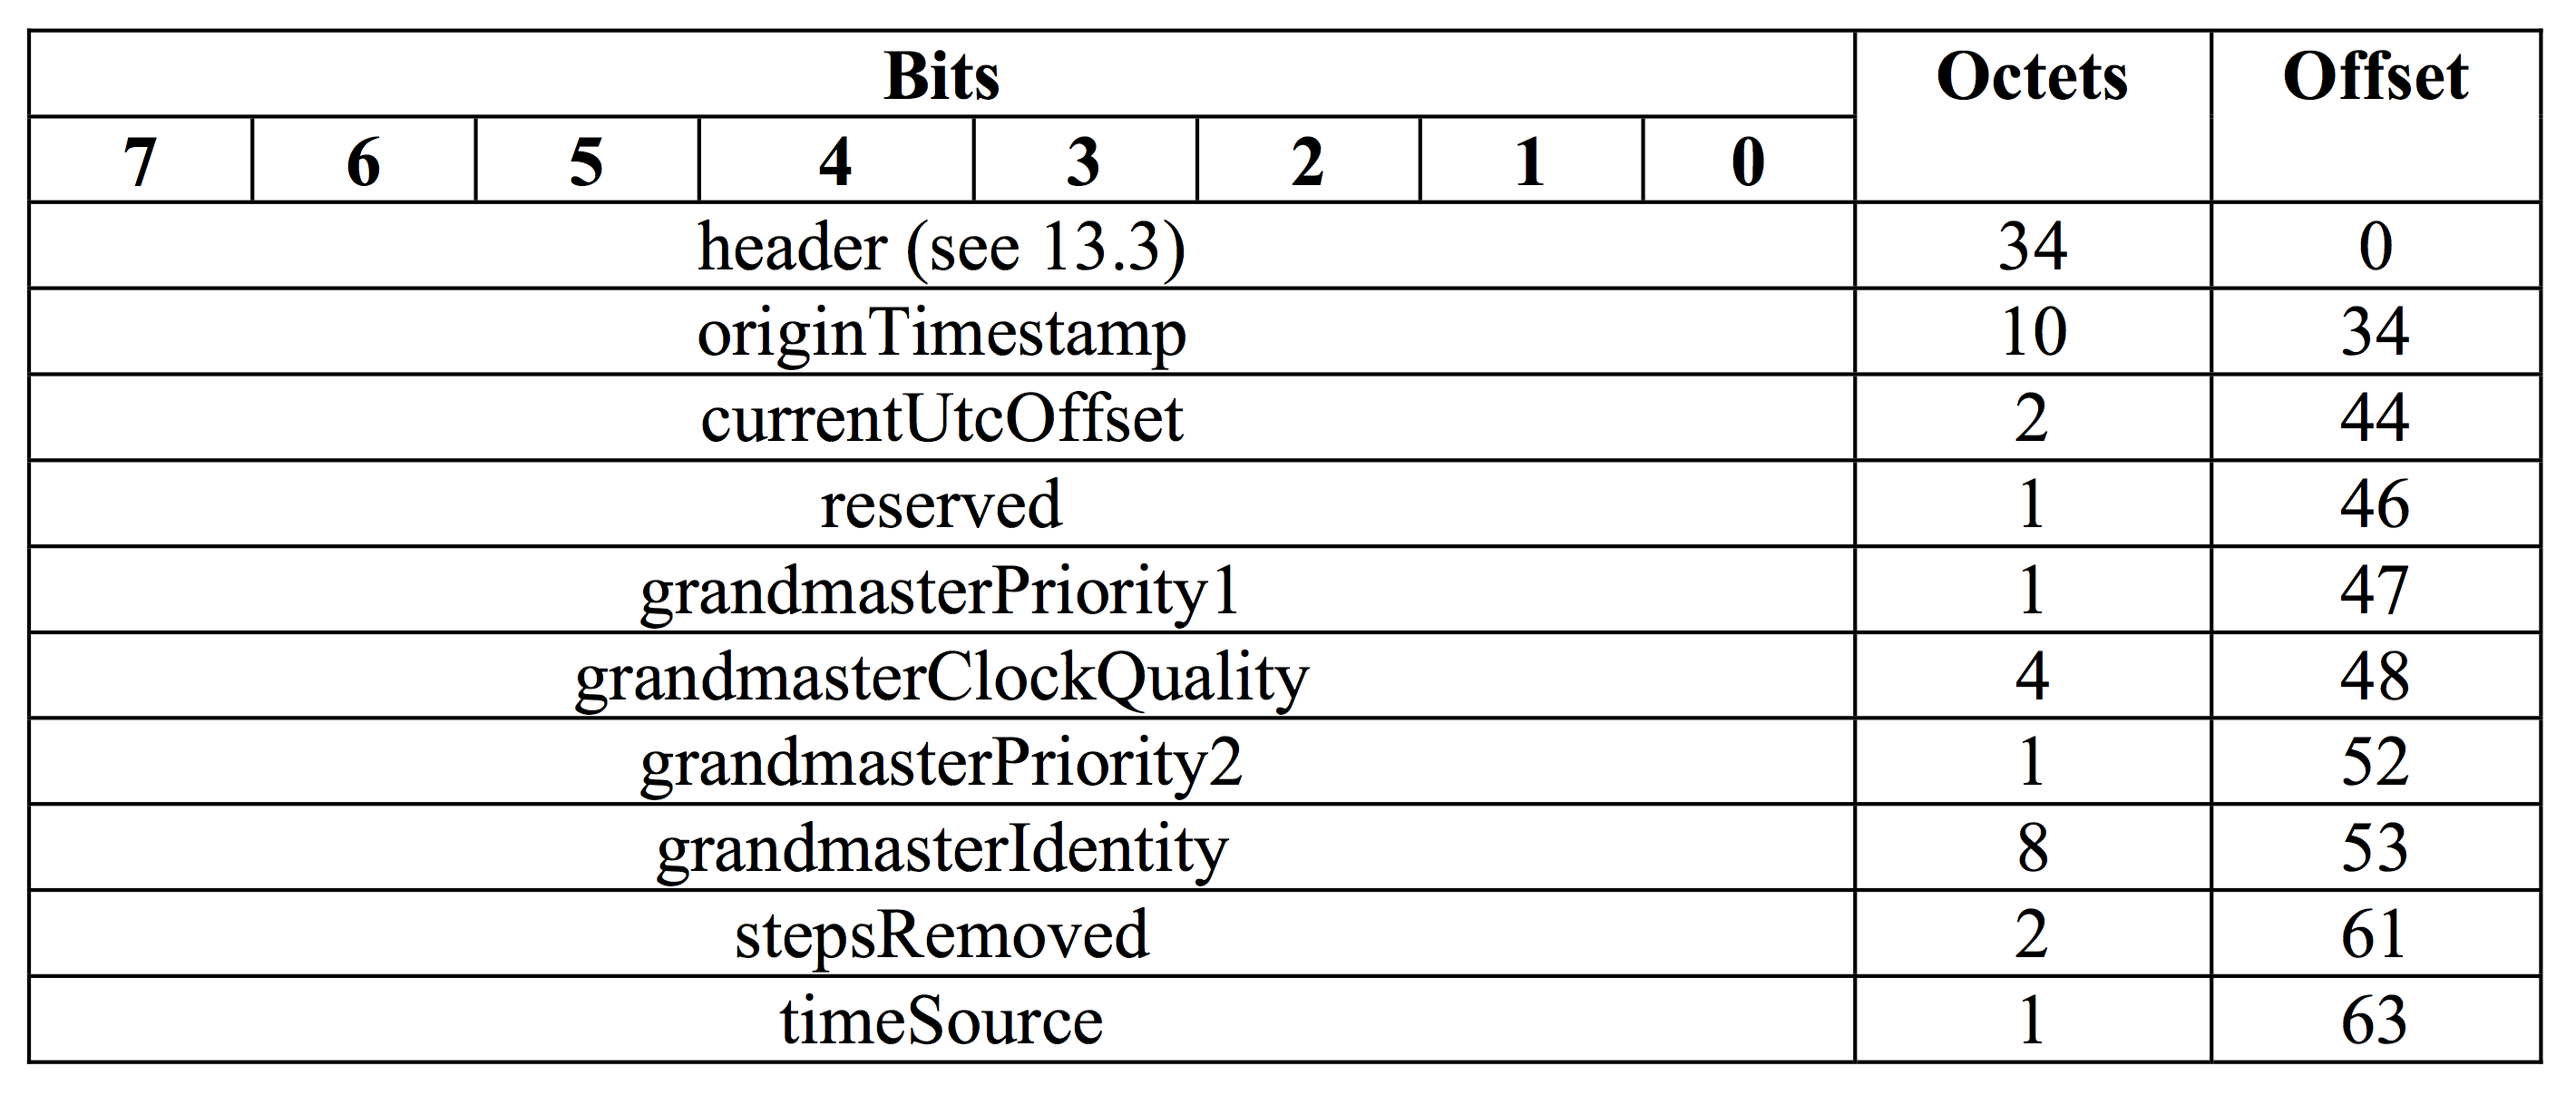
\includegraphics[width=10cm]{ptp_announce_message_content}
%     \bicaption[fig:ptp_announce_message_content]{Announce报文主体格式}{Announce报文主体格式}{Fig}{The Structure of Announce message content}
%   \end{minipage}     
% \end{figure}

% 其中,grandmasterPriority1、grandmasterClockQuality、grandmasterPriority2和grandmasterIdentity等数据都是用来表示Grand Master的时钟质量,对外发送以让其他时钟能够进行数据集比较算法,然后依靠端口状态变化规则来建立整个系统的主从状态。

\section{同步精度的影响因素}
通过对时钟相位、频率同步原理的分析,可以知道整个同步系统会受到多种因素干扰,这些因素不仅会破坏报文传输过程,还会影响到主从时钟频率误差。因此,如果想要实现精确的时钟同步,不仅要利用同步算法把主从时钟偏差计算出来,还需要通过PTP报文的主从传输周期计算出从时钟的频率漂移补偿量。下面对同步过程中破坏相位、频率的因素进行分析。

\subsection{PTP报文传输周期}
在同步过程中,最基本的是$T_{offset}$值和$T_{delay}$值的计算,这将直接影响同步结果的准确性和稳定性,以及最初PTP网络建立的快速性。IEEE1588协议中报文包括事件报文和报文,相关的报文周期和超时事件如下。
\begin{itemize}[noitemsep,topsep=0pt,parsep=0pt,partopsep=0pt]
	\item Announce报文周期:该周期值为$2^{AnnounceInterval}$,协议默认Announce报文默认发送间隔为2s,采用多播方式。当从时钟接收到该报文,若端口为Slave状态,则会更新本地数据集。该报文主要用于最佳主时钟算法,报文内部包含描述主时钟所需的数据集,当时钟接收到该报文时,即会调用最佳主时钟算法,比较自身与外部时钟的品质,并根据结果来决定端口的主从状态\supercite{52}。所以,如果报文周期太长,那么系统建立主从状态则需要花费较多的时间,但如果周期太短,则造成网络拥挤和频繁主从状态刷新。
	\item Sync报文周期:SyncInterval参考值为0.5s-2s。每个Master端口会周期性对外发送Sync报文,该报文包含了主时钟发送时的时间戳。当从时钟接收到该报文,就会通过offset计算方法来计算出主从时间偏差,并以此来校正自身从而实现同步\supercite{52}。如果SyncInterval取值过大,则会使的从时钟偏离太大而失去同步效果;若该周期太小,则会严重加剧网络流量负载,从时钟处于不断的调整波动之中。
	\item Delay\_Req报文周期:MinDelayReqInterval参考值为1s-32s,默认1s。为了获得主从时钟间的路径传输延时,从时钟会周期性对主时钟发送Delay\_Req报文,当主时钟接收到该报文时,会立即保存接收时间戳,并通过回传Delay\_Res报文把接收时间戳返回给从时钟,用于从时钟的$T_{delay}$值更新\supercite{52}如果周期过小,则会给主时钟增加过多的负载压力,加剧网络流量负载;若周期过大,则有可能导致上一次的$T_{delay}$与当前实际$T_{delay}$值出现严重偏差,从而导致$T_{offset}$值偏差较大,严重破坏同步精度。理想的周期应该在区间[0, $2^{MinDelayReqInterval+1}$]中均匀分布。
\end{itemize}

% 首先,一般来讲会在应用层准备PTP协议报文,把当前时间戳信息作为传递数据打包进去并传递给传输层;然后,操作系统按照网络协议栈将应用层数据依次打包进入UDP传输层报文和IP网络层报文;然后从网络层发送给数据链路层,该层会为报文添加以太网帧的首部和尾部形成完整的以太网报文,发送给物理层硬件发送出去\supercite{54}。

% \section{时间序列样本分析及曲线拟合方法}
% 由于在本文中,主要从统计的角度对从时钟处采集到的报文样本进行处理,所以这里对一些常用的序列样本处理方法和曲线拟合方法进行介绍和分析。

% 所谓时间序列样本就是指将系统中某变量的观测值按顺序(周期性)排列成一个数值序列。局部的单个值一般不容易揭示该变量的变化趋势,不过通过把一段时间内的样本累积在一起,就可以很好的展示研究对象在这段时期内的变动过程,然后就可以通过寻找和分析事物的变化特征来计算得出其发展趋势和规律。也能体现系统中某一变量受其它各种因素影响的总结果。

% 在对时间序列样本进行分析的过程中,有一条原则叫作惯性原则,也就是说在一定条件下,被预测事物的过去变化趋势会延续到未来。意味着历史数据存在着某些信息,利用它们可以解释与预测时间序列的现在和未来。另外,通过对样本的统计处理,还能够消除波动因素,使得所有的数据共同构建出一条更为合理的观测曲线。

% 一般而言,时间序列样本具有以下几个特点:
% \begin{itemize}[noitemsep,topsep=0pt,parsep=0pt,partopsep=0pt]
%   \item 趋势性:某个变量随着时间进展或自变量变化,呈现一种比较缓慢而长期的持续上升、下降、停留的同性质变动趋向,但变动幅度可能不等。
%   \item 周期性:某因素由于外部影响随着自然季节的交替出现高峰与低谷的规律。
%   \item 随机性:个别为随机变动,整体呈统计规律。均匀分布、无规则分布,可能符合某统计分布。(用因变量的散点图和直方图及其包含的正态分布检验随机性,大多数服从正态分布。)
%   \item 综合性:实际变化情况一般是几种变动的叠加或组合。预测时一般设法过滤除去不规则变动,突出反映趋势性和周期性变动。
%   \item 平稳性:样本序列的自相关函数在某一固定水平线附近摆动,即方差和数学期望稳定为常数。样本序列的自相关函数只是时间间隔的函数,与时间起点无关。其具有对称性,能反映平稳序列的周期性变化。
% \end{itemize}

% \subsection{时间序列样本处理}
% 首先,要实现时间序列样本建模处理,一般要经过以下几个步骤:

% 1. 利用调查、观测、统计、采样等方法取得被观测系统时间序列动态数据。

% 2. 根据动态数据绘制相关图,通过相关分析计算自相关函数。相关图可以显示变化趋势和周期,发现跳点和拐点。
% \begin{itemize}[noitemsep,topsep=0pt,parsep=0pt,partopsep=0pt]
%   \item 跳点:与其他数据不一致的观测值。如果跳点是正确的观测值,建模时应考虑进去;如果是反常现象,则应把跳点调整到期望值;
%   \item 拐点:时间序列从上升趋势突然变为下降趋势的点。如果存在拐点,则在建模时必须用不同的模型去分段拟合该时间序列,例如采用门限回归模型。
% \end{itemize}

% 3. 利用辨识合适的随机模型来进行曲线拟合,或者说用通用随机模型去拟合时间序列的观测数据。
% \begin{itemize}[noitemsep,topsep=0pt,parsep=0pt,partopsep=0pt]
%   \item 短时间序列:采用趋势模型和季节模型加上误差来进行拟合;
%   \item 平稳时间序列:采用通用ARMA模型(自回归滑动平均模型)及其特殊情况的自回归模型、滑动平均模型或组合-ARMA模型等来进行拟合;
%   \item 非平稳时间序列:先将观测到的时间序列进行差分运算,化为平稳时间序列,再用适当模型去拟合这个差分序列。
% \end{itemize}

% \subsection{常用预测模型}
% 1. 自回归模型,这个模型通过时间序列变量的历史观测值来反映有关因素对预测目标的影响,不受模型变量相互独立的假设条件约束。该模型可消除普通回归预测中自变量选择、多重共线性造成的问题。采用如下的计算方式:
% \begin {align}
% Y_{t} = \phi _{1} * Y_{t-1} + \phi _{2} * Y_{t-2} + ... + \phi _{p} * Y_{t-p} + \varepsilon _{t}
% \end{align}
% 基于假设:$Y_{t}$的变化主要与时间序列的历史数据有关,与其它因素无关;$\varepsilon _{t}$不同时刻互不相关,$\varepsilon _{t}$与$Y_{t}$历史序列不相关。其中,p表示模型的阶次,或者说滞后的时间周期,可以通过实验确定;$Y_{t}$表示当前预测值,与自身过去观测值是同一序列不同时刻的随机变量,相互间有线性关系,也反映时间滞后关系;
% $Y_{t-1}$、...、$Y_{t-p}$是同一平稳序列过去p个时期的观测样本值;然后,$\phi _{1}$、$\phi _{2}$、...、$\phi _{p}$自回归系数,通过计算得出的权数,表达$Y_{t}$依赖于过去的程度,且这种依赖关系恒定不变;$\varepsilon _{t}$随机干扰误差项,均值为零、独立的白噪声序列,通过估计指定的模型获得。

% 2. 移动平均MA(q)模型,基于过去各时期的随机干扰或预测误差的线性组合来计算当前预测值。采用下面计算方式:
% \begin {align}
% Y_{t} = \varepsilon _{t} - \theta _{1} * \varepsilon _{t-1} - ... - \theta _{p} * \varepsilon _{t-p}
% \end{align}

% 3. 自回归移动平均ARMA(p,q)模型,使用两个多项式的比率近似一个较长的AR多项式,即其中p+q个数比 AR(p)模型中阶数p小。前二种模型分别是该种模型的特例。判断预测目标的发展过程与哪一随机过程最为接近。因为只有当样本量足够大时,样本的自相关函数才非常接近母体的自相关函数。采用如下的计算方式:
% \begin {align}
% Y_{t} = \phi _{1} * Y_{t-1} + \phi _{2} * Y_{t-2} + ... + \phi _{p} * Y_{t-p} + \varepsilon _{t} - \theta _{1} * \varepsilon _{t-1} - ... - \theta _{p} * \varepsilon _{t-p}
% \end{align}

% \subsection{曲线拟合}
% 曲线拟合是一种把现有数据透过数学方法来代入一条数式的表示方式。科学和工程问题可以通过采样、实验等方法获得若干离散数据,如果能够找到一个连续的函数(也就是曲线)或者更加密集的离散方程,使得实验数据与方程的曲线能够在最大程度上近似吻合,就可以根据曲线方程对数据进行数学计算,对实验结果进行理论分析,甚至对某些不具备测量条件的位置的结果进行估算。

% 我们一般会通过把离散样本数据来拟合成直线或多项式曲线,从而以一种更加宏观的角度来观察样本数据的变化情况和规律,从而在数学角度预测出更为精确的值。

% 常用的曲线拟合有以下几种方法。

% \subsubsection{最小二乘曲线拟合}
% 这种方法会通过最小化误差的平方和寻找数据的最佳函数匹配,简便地求得未知的数据,并使得所得数据与实际数据之间误差的平方和最小。作为一种插值方法使用时,最小二乘法也可以用于曲线拟合。使用最小二乘法进行曲线拟合理论简单,计算量小,即便是在RBF或三次样条曲线大行其道的今天,最小二乘法在多项式曲线或直线的拟合问题上仍然得到广泛应用。使用最小二乘法,选取的匹配函数的模式非常重要,如果离散数据呈现的是指数变化规律,则应该选择指数形式的匹配函数模式,如果是多项式变化规律,则应该选择多项式匹配模式,如果选择的模式不对,拟合的效果就会很差,这也是使用最小二乘法进行曲线拟合时需要特别注意的一个地方。

% \subsubsection{三次样条曲线拟合}
% 三次样条曲线拟合曲线拟合基本上就是一个插值计算的过程,常用的曲线拟合方法还有基于RBF和三次样条曲线拟合。虽然最小二乘法方法简单,但如果拟合模式不当,会产生较大的偏差,特别是对复杂曲线的拟合。基于RBF的曲线拟合方法需要高深的数学基础,涉及多维空间理论,但是不易得到拟合函数,因此在需要求解拟合函数的情况不是很方便。而三次样条插值是一种工业设计中较为广泛的得到平滑曲线的一种插值方法,可以得到高精度的拟合结果,得到拟合函数。

% \begin{figure}[htbp]
%   \centering
%   \begin{minipage}[b]{0.6\textwidth}
%     \captionstyle{\centering}
%     \centering
%     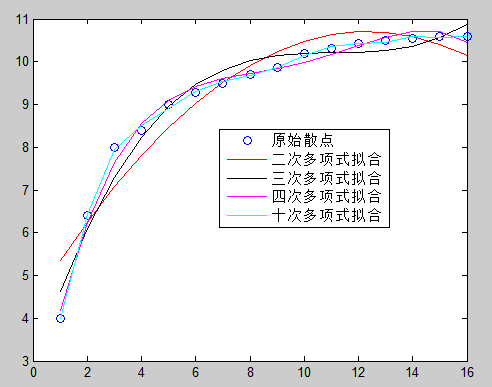
\includegraphics[width=10cm]{三次样条拟合.jpg}
%     \bicaption[fig:Three spline curves fitting]{样条拟合示意图}{样条拟合示意图}{Fig}{The three spline curves fitting}
%   \end{minipage}     
% \end{figure}

% \subsection{IEEE1588实际应用中存在的问题及研究目标}
% 在上文中,主要介绍了IEEE1588协议的实现原理。根据对原理如时钟同步算法的分析研究,再加上PTP协议在工业实际中的精度表现,可以发现该协议中仍然存在一些影响精度的因素,而且,如果希望实际精度能够达到微秒级甚至纳秒级,就不得不对这些因素进行深入的研究。下面将结合IEEE1588的实现原理及实际表现,提出其中存在的固有弊病和漏洞,正是这些问题导致了实际运行中的同步精度难以达到亚微秒级。

\subsection{链路延时不对称}
\label{sec:1588_problem_1}
如式子(2-4)、(2-5)所示,当计算主从时钟偏差$T_{offset}$时,需要先获取链路传输延时$T_{delay}$。在协议中该延时的计算方法是直接假设前后两次传输延时相等,从而通过取平均计算出$T_{offset}$。然而实际上,前后两次的传输路径往往并不对称,即式(2-3)并不成立,而导致往返的链路传输延时不一致的因素\supercite{55}如下。
\begin{itemize}[noitemsep,topsep=0pt,parsep=0pt,partopsep=0pt]
	\item 排队堵塞:当报文在传输中经过中间交换机或路由器时,由于网络负载的不可预知性,无法知道报文在中间交换机上的排队时间,当网络流量良好时,报文可以直接传递过去;而当网络负载较大,可能导致很长的报文排队时间。另外,即使报文可以不用排队,由于协议栈的存在,报文仍然需要经过解包和打包的过程,而这两个过程的消耗时间都与操作系统的调度和协议栈处理过程有关。因此,报文传递过程中穿越交换机时排队和堵塞时间的随机性会导致延时不对称\supercite{46}。
	\item 传输抖动:在网络系统中,所有信息的传递过程所消耗的时间会存在固有的抖动,这是无法避免的。
	\item 网络拓扑结构变化:当拓扑结构突然发生变化,报文传输的路径也就不同了,这必然导致往返链路时延完全不同。
	\item $T_{delay}$与当前真实延时不匹配:因为$T_{delay}$的计算依靠Delay\_Req报文周期,而$T_{offset}$的计算又是依靠Sync报文周期,两者一般并不匹配。所以会导致在计算$T_{offset}$所使用的$T_{delay}$是过去的值,与当前真实的$T_{delay}$值可能并不一致。
\end{itemize}

上述几种现象的存在,都会导致往返的两次延时不一致,所以说,在高同步精度的要求下,真实的传输延时绝对不能简单的假设相等。

\subsection{主从时钟源频率漂移}
由于主时钟在发送Sync报文时的偏差值$T_{offset1}$与从时钟最后接收Delay\_Resp报文时的偏差值$T_{offset2}$是不完全一致的,所以最终计算出来的$T_{offset}$并不完全等于真实的$T_{offset2}$。而且,在实际工业环境中,由于主时钟一般会采用更为稳定、精度较高的设备,而从时钟则一般精度较低,晶振源容易发生漂移现象,从而导致主从时钟之间的频率无法保持一直,这个因素会持续不断的使得从时钟偏离主时钟,因此,本文将对从时钟频率进行补偿,从而降低从时钟漂移现象对同步精度带来的破坏。

\subsection{时间戳的精确度}
\label{sec:1588_problem_2}
对于很多采用软件时间戳方式的设备,报文在协议栈中传递所带来的延时会导致物理层之上的时间戳往往不能真实反映报文的发送时间或接收时间,从而导致时间戳\supercite{53}。这也导致报文封装和解包过程产生偏差,直接破坏最终的时钟同步精度。本交换机项目中,采用的是支持硬件时间戳的设备,即设备能够直接在物理层为报文添加时间戳,从而保证了时间戳的精确度,因此,在本文将会忽略此因素。

\section{本章小结}
本章首先介绍了IEEE1588时钟调频调相的同步原理,并且对其中与本文相关的时钟同步过程进行了分析,另外,还分析了ptp报文传输过程消耗的时间对同步精度的影响,表明了封装中发生的排队堵塞现象和传输中的链路变化等均会严重破坏最终的时钟同步精度。
